%-------------------------------------------------------------------------------
%    SECTION TITLE
%-------------------------------------------------------------------------------
\cvsection{项目经历}


%-------------------------------------------------------------------------------
%    CONTENT
%-------------------------------------------------------------------------------

\cvsubsection{创新创业实践 \& 竞赛项目}

\begin{cventries}
    
%---------------------------------------------------------
\cventry
{主持} % Job title
{智影——基于联邦学习的智慧医疗影像识别系统} % Organization
{中国·海南} % Location
{2020.03 - 至今} % Date(s)
{
    \begin{minipage}[b]{0.25\linewidth}
        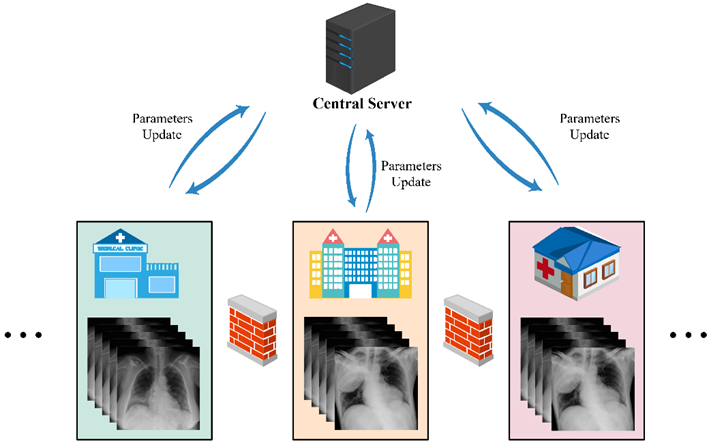
\includegraphics[height=8\baselineskip]{figure/fedcov.png}
    \end{minipage}
    \hfill
    \begin{minipage}[b]{0.7\linewidth}
        我们设计了一款基于联邦学习的医疗影像识别软件,可以在保护患者数据隐私的前提下进行
        多方联合。在数据方面,我们汇总了网上的多个公开数据集,并用Pydicom将dicom文件转
        换成图片形式用于模型识别。在模型方面,我们将包括ResNet、COVID-Net在内的4个模型
        进行模型融合,增强系统稳定性和泛化能力。同时,我们用GradCAM++对卷积层进行可视化,
        用于标记病灶位点,最后能够自动化生成医学报告。另外,在多方贡献衡量方面我们提出
        了FedCM贡献评估算法。\textcolor{awesome-red}{\href{https://github.com/beiyuouo/paddle-fl-gui}{[Code]}}
    \end{minipage}
}

%---------------------------------------------------------
\cventry
{参与} % Job title
{基于5G和多维传感的无人驾驶城市巡逻车} % Organization
{中国·海南} % Location
{2020.05 - 至今} % Date(s)
{
    \begin{minipage}[b]{0.25\linewidth}
        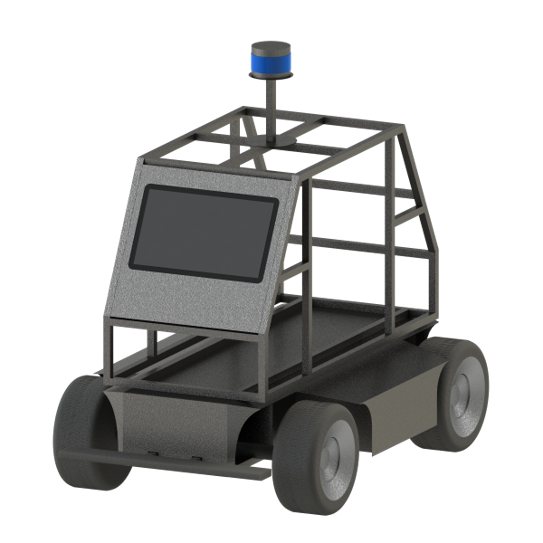
\includegraphics[height=8\baselineskip]{figure/car.png}
    \end{minipage}
    \hfill
    \begin{minipage}[b]{0.7\linewidth}
        我们设计了一款基于5G和多传感器融合用于城市巡逻的无人路检机器人,主要
        功能有基于多传感器融合的道路裂缝、坑洼等缺陷检测并进行云端上报,和违
        停检测。在建图和定位方面,我们基于LeGO-LOAM进行调整和改进。在道路检
        测方面,我们基于YOLOv5训练了自己的模型,F1-score达到了0.68。
    \end{minipage}
}

%---------------------------------------------------------
\cventry
{参与} % Job title
{基于ROV技术的水下观光机器人设计及其VR实时观景功能实现} % Organization
{China} % Location
{2020.05 - 至今} % Date(s)
{
    这是一个国家级大学生创新创业实训项目。我们利用水下ROV进行图像的采集和传输,在降噪去雾之后,
    对视频序列进行拼接,以实现全景景观的观看。
}

%---------------------------------------------------------
%\end{cventries}

%\cvsubsection{Open Source Project}

%\begin{cventries}
%---------------------------------------------------------
%    \cventry
%    {Owner} % Job title
%    {FedMedical:PaddleFL-based Federated Learning Medical Image Recognition Software} % Organization
%    {\href{https://github.com/beiyuouo/paddle-fl-gui}{\color{awesome-red}{[GitHub link]}}} % Location
%    {2020.11 - PRESENT} % Date(s)
%    {
%        \begin{cvitems} % Description(s) of tasks/responsibilities
%            \item {Distributed Deployment and Federated Learning Simultaneous Training with PaddleFL Framework.}
%        \end{cvitems}
%    }

%---------------------------------------------------------
\cventry
%    {项目所有者} % Job title
%    {凌空画笔:基于YOLOv5和OpenCV的手势识别和跟踪} % Organization
%    {\href{https://github.com/beiyuouo/mid-air-draw}{\color{awesome-red}{[GitHub link]}}} % Location
%    {2020.09 - PRESENT} % Date(s)
%    {
%        \begin{cvitems} % Description(s) of tasks/responsibilities
%            \item {利用YOLOv5进行手势识别和手部关键点识别和跟踪,用OpenCV展示结果并进行图像绘制}
%        \end{cvitems}
%    }
{项目拥有者} % Job title
{凌空画笔:基于YOLOv5和OpenCV的手势识别和跟踪} % Organization
{中国·海南} % Location
{2020.09 - 至今} % Date(s)
{
    我们自己收集和标注的数据,并利用YOLOv5进行手势的识别和手指关键点的识别。
    可以利用它与PPT等软件进行绘制和交互。\textcolor{awesome-red}{\href{https://github.com/beiyuouo/mid-air-draw}{[Code]}} \textcolor{awesome-red}{\href{https://www.bilibili.com/video/BV15V411a7WB/}{[Video]}}
}

%---------------------------------------------------------
%  \cventry
%    {主持 \& 参与} % Job title
%    {大学生创新创业实践项目} % Organization
%    {中国·海南} % Location
%    {2020.05 - 至今} % Date(s)
%    {
%      \begin{cvitems} % Description(s) of tasks/responsibilities
%        \item {基于联邦学习框架下对新冠病毒CXR医疗影像识别系统的研究}
%        \item {基于ROV技术的水下观光机器人设计及其VR实时观景功能实现}
%      \end{cvitems}
%    }

%---------------------------------------------------------
%    \cventry
%    {主持} % Job title
%    {智影——基于联邦学习的智慧医疗影像识别系统} % Organization
%    {中国·海南} % Location
%    {2020.03 - 至今} % Date(s)
%    {
%        \begin{cvitems} % Description(s) of tasks/responsibilities
%            \item {开发了一款基于联邦学习框架的医疗影像识别软件,并提供GUI界面}
%            \item {扩充和汇总多个肺部影像数据集,可以识别多达10种肺部病症}
%            \item {利用多模型融合方法提高系统稳定性}
%            \item {利用Grad-CAM++对病灶位点进行标注,并自动化生成报告}
%            \item {利用提出的FedCM方法对每个医疗机构贡献进行评估}
%        \end{cvitems}
%    }
%
%---------------------------------------------------------
%    \cventry
%    {参与} % Job title
%    {5G无人驾驶城市巡逻车} % Organization
%    {中国·海南} % Location
%    {2020.05 - 至今} % Date(s)
%    {
%        \begin{cvitems} % Description(s) of tasks/responsibilities
%            \item{利用YOLOv5进行路面裂缝检测和行人检测}
%            \item{利用OpenCV和SVM进行车牌照检测和识别}
%        \end{cvitems}
%    }
%
%---------------------------------------------------------
\end{cventries}

%\cvsubsection{开源项目}

%\begin{cventries}
%---------------------------------------------------------
%    \cventry
%    {项目所有者} % Job title
%    {FedMedical:基于PaddleFL的联邦学习医疗影像识别软件} % Organization
%    {\href{https://github.com/beiyuouo/paddle-fl-gui}{\color{awesome-red}{[GitHub link]}}} % Location
%    {2020.11 - PRESENT} % Date(s)
%    {
%        \begin{cvitems} % Description(s) of tasks/responsibilities
%            \item {利用PaddleFL框架实现分布式部署和联邦学习同步训练}
%        \end{cvitems}
%    }

%---------------------------------------------------------
%    \cventry
%    {项目所有者} % Job title
%    {凌空画笔:基于YOLOv5和OpenCV的手势识别和跟踪} % Organization
%    {\href{https://github.com/beiyuouo/mid-air-draw}{\color{awesome-red}{[GitHub link]}}} % Location
%    {2020.09 - PRESENT} % Date(s)
%    {
%        \begin{cvitems} % Description(s) of tasks/responsibilities
%            \item {利用YOLOv5进行手势识别和手部关键点识别和跟踪,用OpenCV展示结果并进行图像绘制}
%        \end{cvitems}
%    }
%

%---------------------------------------------------------
%\end{cventries}

